\documentclass{article}
\usepackage{graphicx}
\usepackage{mathtools}
\begin{document}
	\section*{Lsg Vorschlag D+S Ü011 Maximilian Maag}
	\section*{Aufgabe A}
	\subsection*{a)}
	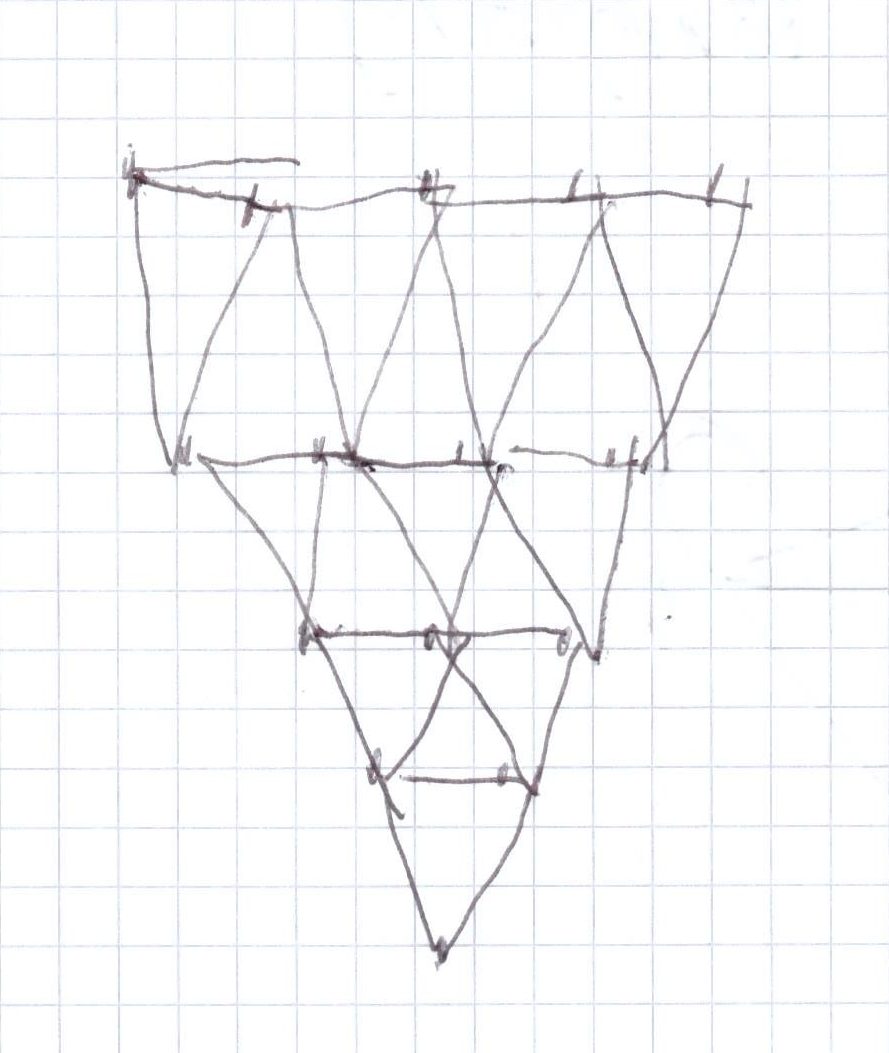
\includegraphics[width=\linewidth]{11A} \\
	Die gezeigte Skizze dient nur zur Verdeutlichung und ist nicht maßstabsgerecht.
	\subsection*{b)}
	Der Grad aller Knoten ist gerade. Es handelt sich um eulersche Graphen.
	\subsection*{c)}
	Von Außen nach Innen. Vergleich Haus vom Nikolaus.
	\section*{Aufgabe B}
	$K_5$: Es muss mindestens 1 Kante entfernt werden. \\
	
	\section*{Aufgabe C}
	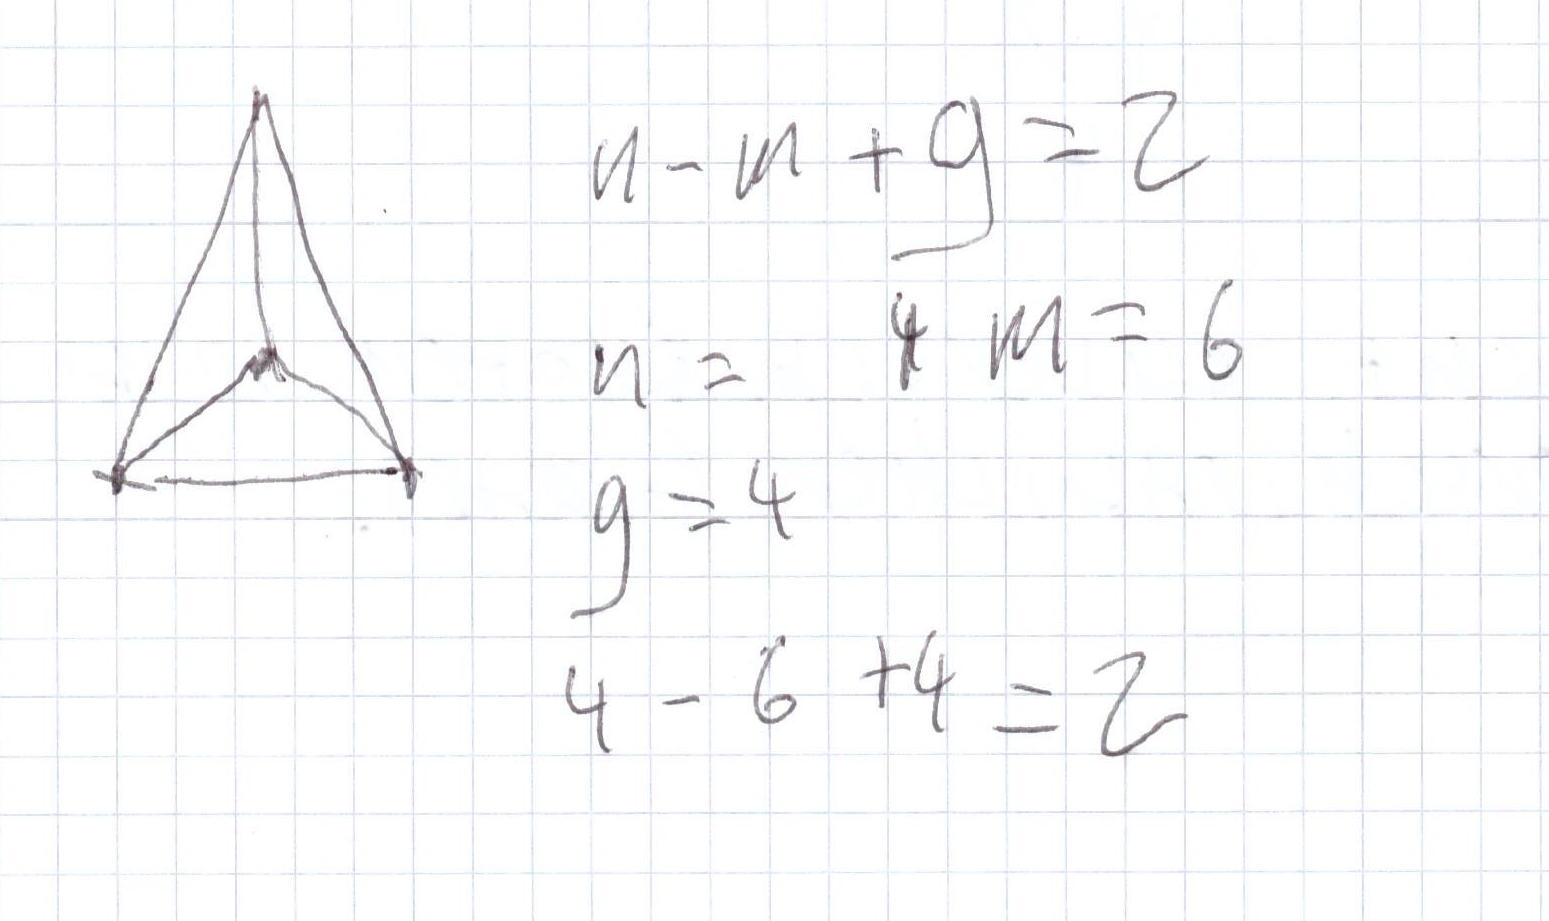
\includegraphics[width=\linewidth]{11C}
	\section*{Aufgabe 1}
	\subsection*{a)}
	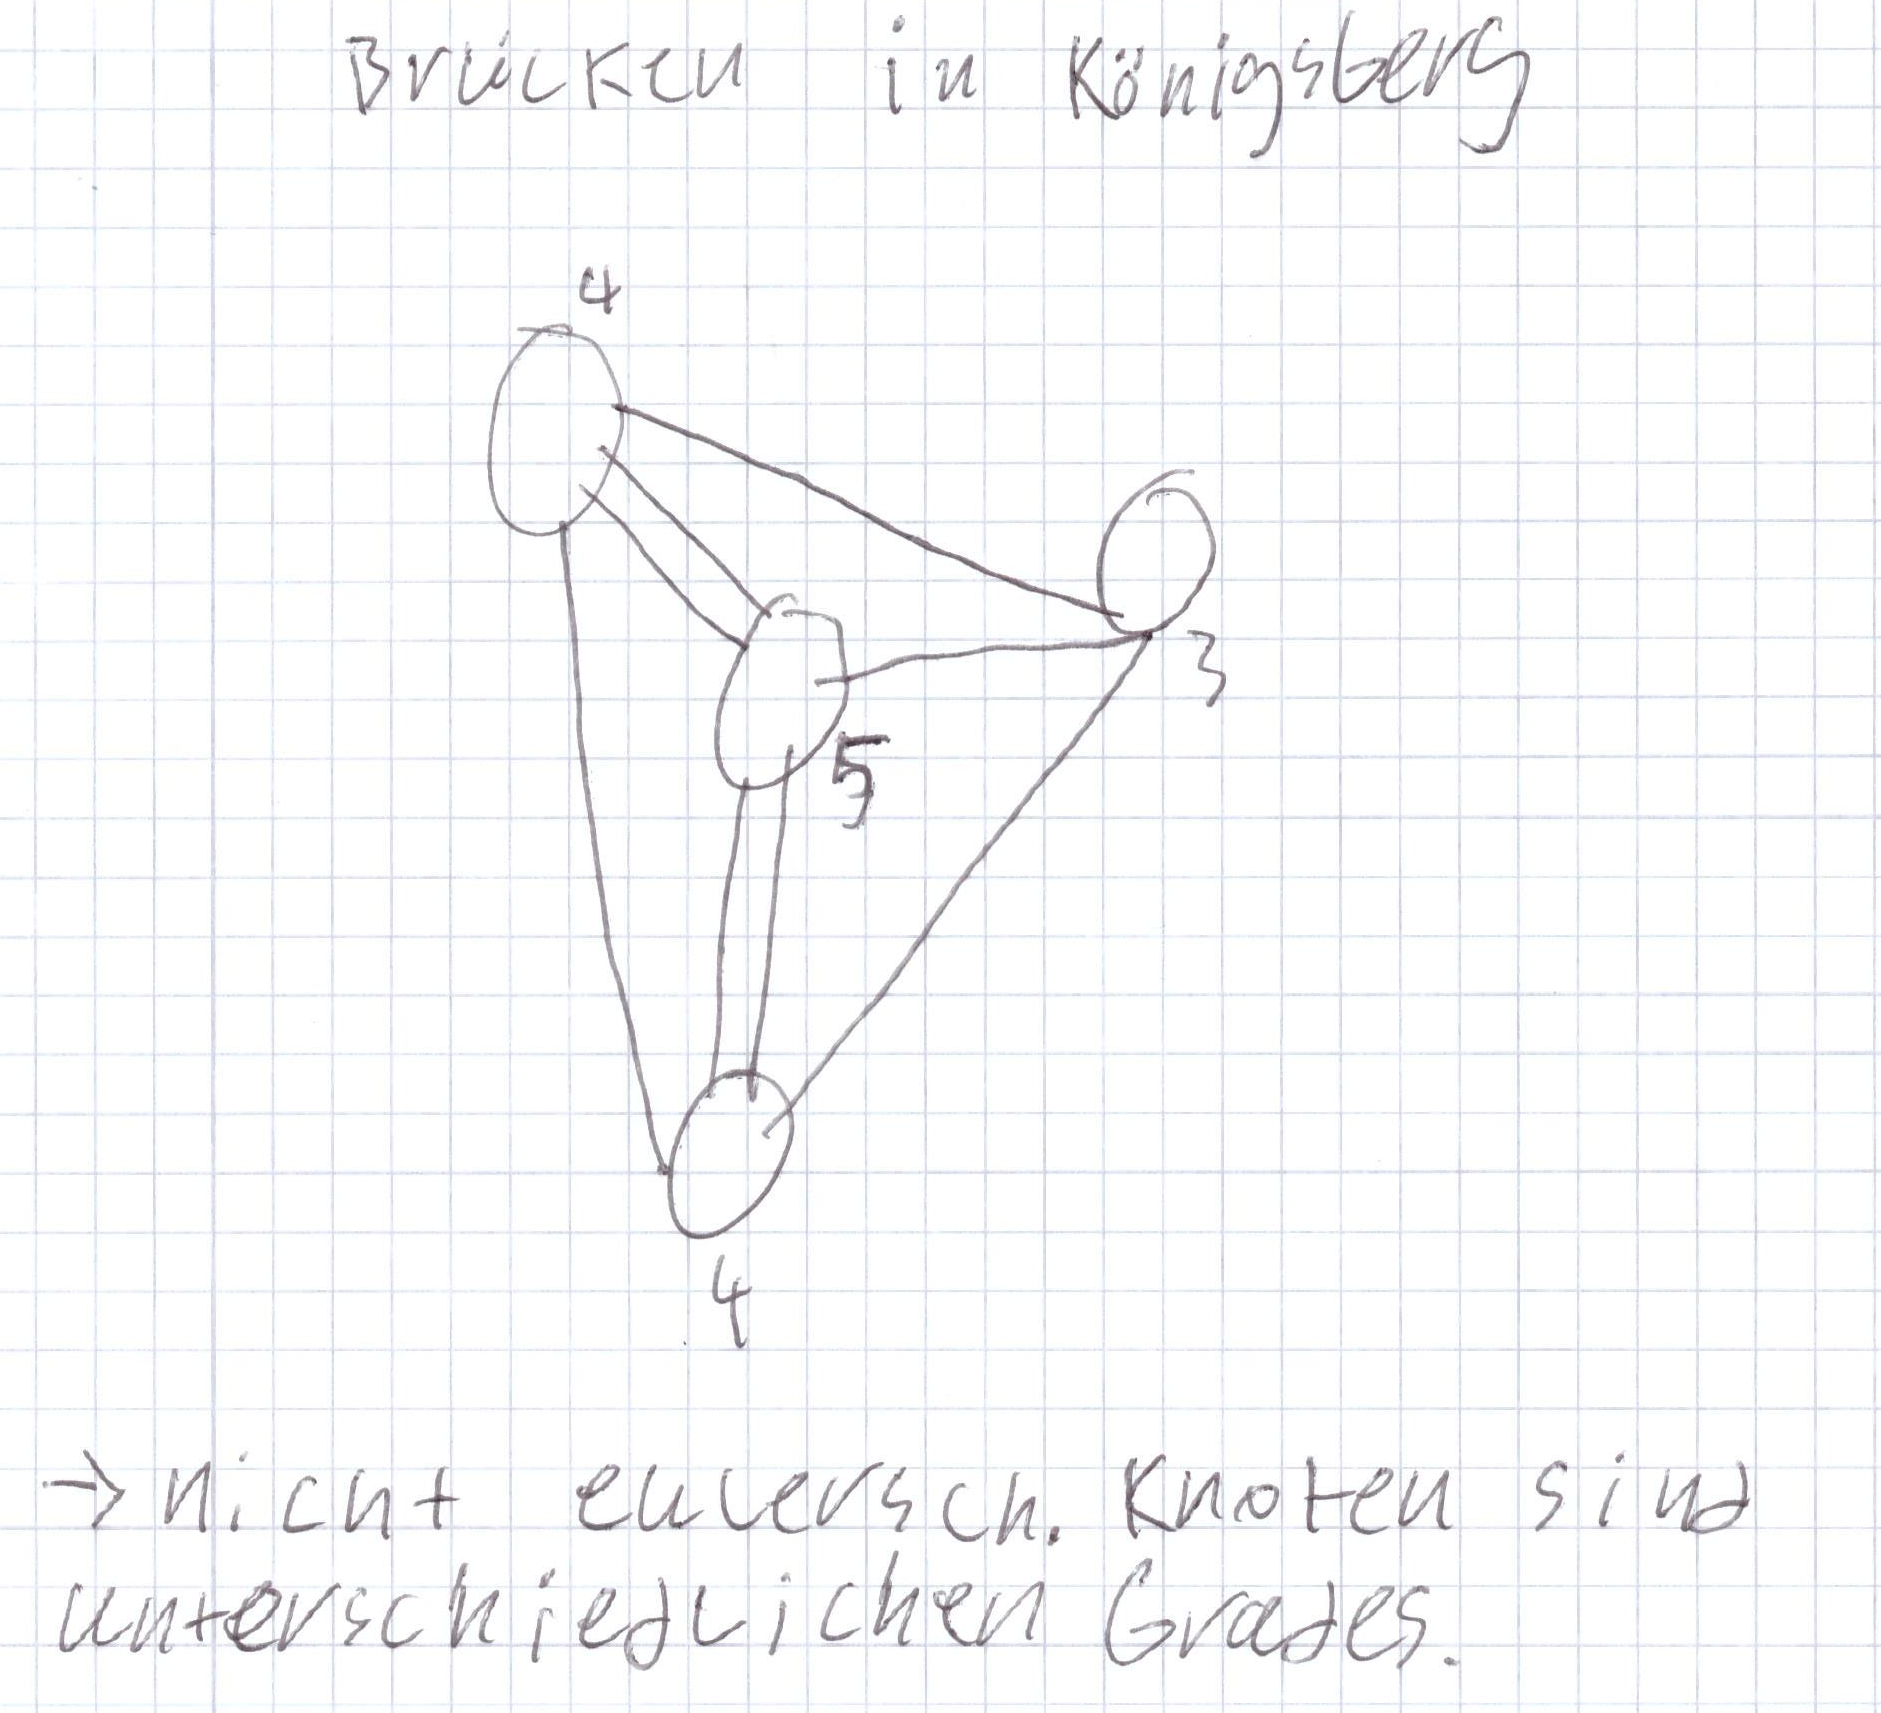
\includegraphics[width=\linewidth]{111a}
	\subsection*{b)}
	Der mittlere und der rechte Knoten haben einen unterschiedlichen Grad, daher kann der Graph nicht eulersch sein.
	\subsection*{c)}
	Es gibt zwei Knoten ungeraden Grades, dadurch enthält der Graph auch eine offene eulersche Linie.
	
	\section*{Aufgabe 2}
	$n - m + g = 2$
	\begin{tabular}[h]{c|c|c}
		n & m & g \\
		\hline
		10&9&1 \\
		5&8&5 \\
		9&11&4 
		
	\end{tabular}
	\section*{Aufgabe 3}
	Def. \\
	$\bigwedge_{i = 1}^{n} A_i \equiv A_1 \land A_2 ... \land A_n $ \\
	$\bigvee_{i = 1}^{n} A_i \equiv A_1 \lor A_2 ... \lor A_n$ \\ \\
	Zu Zeigen: \\
	$\not(\bigwedge_{i = 1}^{n} A_i) \equiv \bigvee_{i = 1}^{n} \not A_i$ \\ \\
	Basis: n = 1 \\
	$\not(\bigwedge_{i = 1}^{1} A_1) \equiv \bigvee_{i = 1}^{1} \not A_1$ \\
	$\not A_1 \equiv \not A_1$ \\ \\
	Schritt: n $\to$ n+1 \\
	$\not A_1 \land \not A_2 \land \not A_3 ... \land \not A_n \land \not A_{n+1} \equiv \not A_1 \lor \not A_2 \lor \not A_3 ... \lor \not A_n \lor \not A_{n+1}$ \\
	$\not(\bigwedge_{i = 1}^{n} A_i) \land \not A_{n+1} \equiv \bigvee_{i = 1}^{n} \not A_i \lor  \not A_{n+1}$ \\
	$\not(\bigwedge_{i = 1}^{n+1} A_i) \equiv \bigvee_{i = 1}^{n+1} \not A_i$ \\
	q.e.d.
\end{document}